\chapter{Solución propuesta}
\label{solucion}
En la actualidad el desarrollo de Internet ha alcanzado niveles realmente impresionantes, no solo en lo que respecta a avances en capacidad de transmisión y almacenamiento de datos sino también en su modelo de crecimiento y expansión en la sociedad post-moderna en la era de la información. Prácticamente no hay rincón del planeta en donde no pueda hoy en día llegar la red de redes\cite{iternet}.\\

\section{Arquitectura de la solución}
\label{arquitectura}
De acuerdo al problema planteado y a los requerimientos especificados en el capítulo \ref{alcances}, es esencial implementar un sistema que pueda difundirse en la sociedad de manera masiva y veloz. La RedSolLAC quiere y debe poder llegar al mayor número de personas interesadas en producir energías limpias y renovables.\\

Actualmente la RedSolLAC solo cuenta con un sitio Web donde publica información respecto de plantas solares productoras de energía, sin embargo con el objetivo de expandir sus alcances, objetivos y adherir miembros a la red, es que requiere de nuevas herramientas atractivas para los futuros integrantes. Es acá donde la presente memoria interviene, para desarrollar un nuevo sistema que integre el sitio Web ya existente con nuevas componentes que marquen la diferencia.

Para dar cumplimiento a los requerimientos se propone la siguiente arquitectura:

\begin{figure}[h!]
        \centering
        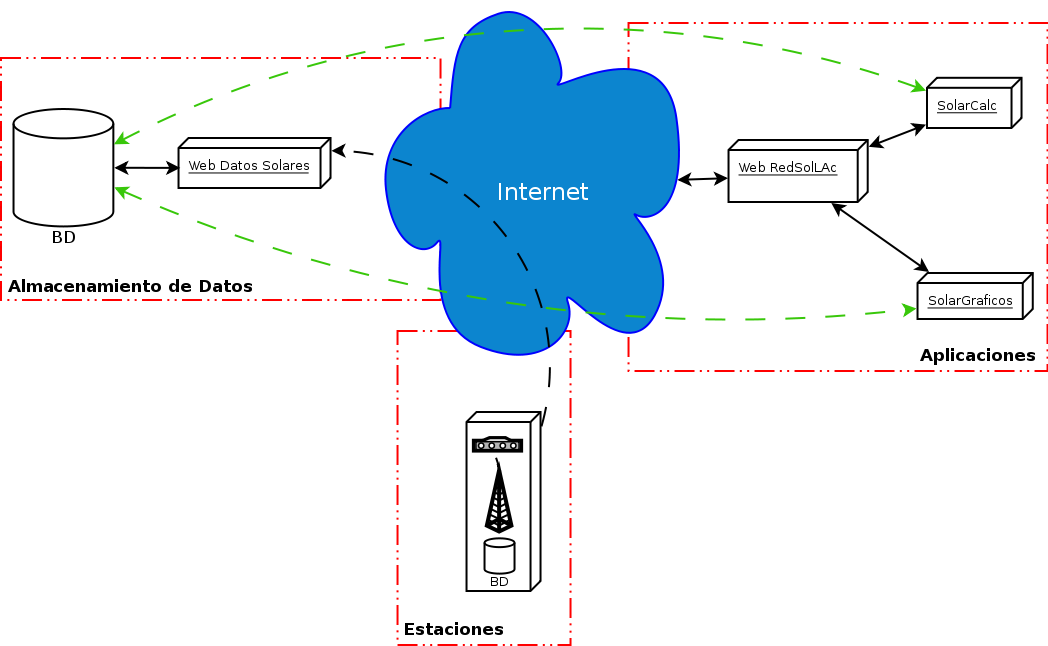
\includegraphics[width=400pt]{images/diagramaArquitectura}
        \caption{Diagrama general de arquitectura.}
	\label{da}
\end{figure}

En el diagrama (Fig:\ref{da}) apreciamos las 3 partes que componen el nuevo sistema desarrollado, en primer lugar la componente de ''Aplicaciones'', consiste en un servidor Web que implementa la plataforma CMS Wordpress. Bajo esta plataforma se desarrollan las aplicaciones principales del sistema, que serán visitadas por los usuarios finales. Luego tenemos las ''Estaciones meteorológicas'', que son parte fundamental del proceso de adquisición de datos, cada una de ellas cuenta con diferentes sensores que miden el medio donde están instaladas. A través de un sistema de comunicación envían los datos a la plataforma de almacenamiento de datos. Finalmente la componente de ''Almacenamiento de Datos'', la cual consiste en un servidor Web que administra los procesos de registro, acceso y mantención de datos y un servidor de base de datos. Cada una de estas partes debe interactuar con las demás de manera muy precisa para conseguir el comportamiento requerido.\\

A continuación se describen las diferentes herramientas tanto de hardware como de software que permiten implementar el sistema:

\subsection{Software utilizado}
\subsubsection{Wordpress}
Wordpress es una avanzada plataforma semántica de publicación en la Web; libre, de código abierto y gratuito\footfullcite{foot:softwarelibre,} con altos estándares de diseño y usabilidad. Es un sistema de manejador de contenidos (\gloss{cms}) basado en estilo de publicación de blogs. Se distribuye bajo la licencia GPL. Está escrito en lenguaje PHP, utiliza el motor de bases de datos MySql y hojas de estilo CSS para la parte visual. Su arquitectura está pensada y diseñada de forma modular, lo que le permite adaptarse y ser configurable de acuerdo con los requerimientos de cada usuario.\\

La primera versión fue liberada el año 2003 por Matt Mullenweg y es un rama de otro proyecto llamado b2/cafelog. Actualmente esta plataforma está en su versión 3.0. Se estima que Wordpress a la fecha es la herramienta de publicación de contenido más utilizada y popular de la Red, con aproximadamente un 14\% de participación en Internet y con más del 22\% de utilización sitios nuevos o que se publican por primera vez\cite{software:usoWordpress}.\\

Wordpress está echo de tal manera que permite a sus usuarios modificar o configurar partes esenciales del sistema, lo que lo hace flexible para agregar funcionalidades y adaptarse a los requerimientos de los usuarios. Además cuanta con un framework y una \gloss{api} que facilita la labor de los programadores.\\

\newpage
Algunas características específicas de Wordpress son:

\paragraph{Perfil Gráfico:}	
La parte visual de esta plataforma funciona a través de un sistema llamado ''\gloss{themes}\footfullcite{foot:themes}'' (para efectos prácticos en adelante ''Perfiles''). Los ''Perfiles'' son un conjunto de bibliotecas programadas en PHP y JavaScript que permiten organizar la forma en que se presentan los contenidos del sitio sin alterar este mismo. Wordpress al estar diseñado de manera modular, permite a sus usuarios contar con gran cantidad de ''Perfiles'' diferentes. Mediante una interfaz de administración permite cambiar estos "Perfiles" de manera rápida y sencilla. Adicionalmente en el mercado, existen extensos depósitos de ''Perfiles'' que pueden ser instalados en cualquier sitio compatible con la versión indicada por el programador.
En el sitio de Wordpress se puede encontrar una extensa documentación y una API que indica a los programadores que deseen desarrollar nuevos ''Perfiles'', cómo deben estructurar los ficheros y qué funcionalidades pueden agregar o quitar. Adicionalmente, los ''Perfiles'' pueden publicarse o bien Wordpress da la libertad a sus usuarios de vender trabajos basados en su framework, es decir, que éstos quedan en la libertad de licenciar sus códigos como mejor lo estimen conveniente.

\paragraph{Plugins:}
Los ''\gloss{plugins}\footfullcite{foot:plugins}''  funcionan casi de la misma manera que los ''Perfiles'' y así también la mayoría de los componente que dispone Wordpress. Estos son un conjunto de bibliotecas\footfullcite{foot:bibliotecas} programadas en PHP y JavaScript que pueden instalarse o desinstalares desde el panel de administración.\\
Cada ''Plugin'' está diseñado para agregar nuevas funcionalidades o modificar el comportamiento normal de los sitios. La documentación de Wordpress entrega pautas estrictas de cómo deben estar programadas las bibliotecas para que las nuevas funcionalidades no interfieran con el funcionamiento normal del sistema.

\paragraph{Widgets:}
Los ''Widgets'' son pequeños programas autónomos, que permiten agregar nuevas funcionalidades al sistema, pero que a diferencia de un ''Plugin'' común y corriente poseen una interfaz visual y están diseñados para exponer al usuario algún dato o funcionalidad específica. Estos pequeños programas pueden agregarse y quitarse de manera muy rápida, además tienen la característica de ser móviles. Generalmente son programas que se agregan en las barras laterales.

\paragraph{Multiusuario:}
Wordpress permite la creación y administración de muchos usuarios, los cuales pueden tener diferentes responsabilidades dentro del sistema, tales como administrar el contenido o bien la configuración del sitio. Esto permite que la mantención del sitio y a la vez las responsabilidades, puedan estar muy bien distribuidas sin riesgo de que algún usuario realice tareas no permitidas por su nivel de acceso.

\subsubsection{PHP}
PHP es un acrónimo recursivo que significa ''PHP Hypertext Pre-processor''. Fue creado originalmente por Rasmus Lerdorf en 1994; sin embargo, la implementación principal de PHP es liderada , en la actualidad por ''The PHP Group\cite{php:1}''. Publicado bajo la PHP License. La ''Free Software Foundation'' considera esta licencia como software libre.\\

Es un lenguaje de programación interpretado de alto rendimiento, diseñado originalmente para la creación de páginas web dinámicas. Se usa principalmente para la interpretación del lado del servidor (server-side scripting), pero actualmente puede ser utilizado desde una interfaz de línea de comandos o en la creación de otros tipos de programas incluyendo aplicaciones con interfaz gráfica. Sus características principales son:

\begin{itemize}
\item Orientado al desarrollo de aplicaciones web dinámicas con acceso a información almacenada en una base de datos.
\item El código fuente escrito en PHP es invisible al navegador web y al cliente, ya que es el servidor el que se encarga de ejecutar el código y enviar su resultado HTML al navegador. Esto hace que la programación en PHP sea segura y confiable.
\item Capacidad de conexión con la mayoría de los motores de base de datos que se utilizan en la actualidad, destaca su conectividad con MySQL y PostgreSQL.
\item Capacidad de expandir su potencial utilizando módulos.
\item Posee una amplia documentación en su sitio web oficial, entre la cual se destaca que todas las funciones del sistema están explicadas y ejemplificadas en un único archivo de ayuda.
\item Es libre, por lo que se presenta como una alternativa de fácil acceso para todos.
\item Permite aplicar técnicas de programación orientada a objetos.
\item Amplia biblioteca nativa de funciones.
\item No requiere definición de tipos de variables aunque sus variables se pueden evaluar también por el tipo que estén manejando en tiempo de ejecución.
\item Tiene manejo de excepciones (desde PHP5).
\item Si bien PHP no obliga a quien lo usa a seguir una determinada metodología a la hora de programar (muchos otros lenguajes tampoco lo hacen), aun haciéndolo, el programador puede aplicar en su trabajo cualquier técnica de programación o de desarrollo que le permita escribir código ordenado, estructurado y manejable. Un ejemplo de esto son los desarrollos que en PHP se han hecho del patrón de diseño Modelo Vista Controlador (MVC), que permiten separar el tratamiento y acceso a los datos, la lógica de control y la interfaz de usuario en tres componentes independientes.
\end{itemize}

\subsubsection{MySQL}
	MySQL es un sistema de gestión de bases de datos relacional, multihilo y multiusuario con más de seis millones de instalaciones. MySQL AB desde enero de 2008 una subsidiaria de Sun Microsystems y ésta a su vez de Oracle Corporation desde abril de 2009, desarrolla MySQL como software libre en un esquema de licenciamiento dual. Por un lado, se ofrece bajo la \gloss{gnu} GPL para cualquier uso compatible con esta licencia, pero para aquellas empresas que quieran incorporarlo en productos privativos deben comprar a la empresa una licencia específica que les permita este uso. Está desarrollado en su mayor parte en \gloss{ansic}.\\

Al contrario de proyectos como Apache, donde el software es desarrollado por una comunidad pública y los derechos de autor del código están en poder del autor individual, MySQL es patrocinado por una empresa privada, que posee el copyright de la mayor parte del código.\\
Esto es lo que posibilita el esquema de licenciamiento anteriormente mencionado. Además de la venta de licencias privativas, la compañía ofrece soporte y servicios. Para sus operaciones contratan trabajadores alrededor del mundo que colaboran vía Internet. MySQL AB fue fundado por David Axmark, Allan Larsson y Michael Widenius. Sus características principales son:

\begin{itemize}
\item Usa GNU Automake, Autoconf, y Libtool para portabilidad.
\item Uso de multihilos mediante hilos del kernel.
\item Usa tablas b-tree para búsquedas rápidas con compresión de índices.
\item Usa tablas hash en memoria temporales.
\item El código MySQL se prueba con Purify (software comercial) detector de memoria perdida así como con Valgrind (una herramienta GPL).
\item Completo soporte para operadores y funciones de selección.
\item Completo soporte de funciones de agrupación
\item Ofrece un sistema de seguridad de contraseñas y privilegios mediante verificación basada en el host y el tráfico de contraseñas está cifrado al conectarse a un servidor.
\item Soporta gran cantidad de datos (hasta 50 millones de registros).
\item Se permiten hasta 64 índices por tabla (32 antes de MySQL 4.1.2). Cada índice puede consistir desde 1 hasta 16 columnas o partes de columnas y el tamaño máximo son 1000 bytes (500 antes de MySQL 4.1.2).
\item Los clientes se conectan al servidor MySQL usando ''\gloss{sockets}'' ''\gloss{tcpip}'' en cualquier plataforma.
\item En MySQL 5.0, los clientes y servidores Windows se pueden conectar usando memoria compartida.
\item MySQL contiene su propio paquete de pruebas de rendimiento proporcionado con el código fuente de la distribución de MySQL.
\end{itemize}

\subsubsection{CSS}
\gloss{css} es un lenguaje usado para definir la presentación de un documento estructurado escrito en HTML o XML. El \gloss{w3c} es el encargado de formular la especificación de las hojas de estilo que servirán de estándar para los agentes de usuario o navegadores.\\
La idea que se encuentra detrás del desarrollo de CSS es separar la estructura de un documento de su presentación. La información de estilo puede ser adjuntada como un documento separado o en el mismo documento HTML. En este último caso podrían definirse estilos generales en la cabecera del documento o en cada etiqueta particular.

\subsubsection{jQuery}
jQuery\cite{software:jquery} es una biblioteca de JavaScript, creada inicialmente por John Resig, que permite simplificar la manera de interactuar con los documentos HTML, manipular el árbol \gloss{dom}, manejar eventos, desarrollar animaciones y agregar interacción con \gloss{ajax} a páginas web. Fue presentada el 14 de enero de 2006 en el BarCamp \gloss{nyc}. Es software libre y de código abierto, posee un doble licenciamiento bajo la Licencia MIT\cite{licencia:mit} y la Licencia Pública General de GNU\cite{licencia:gnu}, permitiendo su uso en proyectos libres y privativos. jQuery, al igual que otras bibliotecas, ofrece una serie de funcionalidades basadas en JavaScript que de otra manera requerirían de mucho más código, es decir, con las funciones propias de esta biblioteca se logran grandes resultados en menos tiempo y espacio.
Para incrementar la funcionalidad de jQuery se le agregaron algunos plugins como Flot\cite{software:flot} que permite crear de manera sencilla gráficos a partir de conjuntos de pares de datos.

\subsection{Hardware}
Durante el desarrollo e implementación del software involucrado en esta Memoria, fue necesario interiorizarse con una serie de elementos de hardware que forman parte de la mayoría de las estaciones meteorológicas para plantas de energía solar, así como elementos comunes empleados en la construcción de estas mismas.

\paragraph{Datalogger Campbell CR1000:}
Un Datalogger es un pequeño computador que cuenta con diferentes entradas para la conexión de sensores y otros equipos electrónicos tales como, módems, teclados y/o pantallas. Además cuenta con un sistema operativo que permite ingresar scripts para controlar su funcionamiento.\\El ''datalogger'' CR1000 es compacto y ligero tiene una velocidad de ejecución de programa de 100 Hz y 1.500 Hz en ''burstmode''. En su interior, un procesador de 16-bit H8S Hitachi con 32-bit en la arquitectura interna de la CPU.
Ocho entradas analógicas diferenciales (16 single-ended), dos canales contadores
de pulsos y ocho puertos digitales I/O ports complementados con los puertos CS I/O y RS-232, puerto de 40-pin para periféricos y opción Ethernet (Fig:\ref{cr1000}).

\begin{figure}[h!]
	\centering
	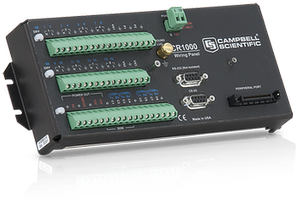
\includegraphics[width=200pt]{images/cr1000}
	\caption{Datalogger Campbell CR1000}
	\label{cr1000}
\end{figure}

Campbell Scientific es una compañía dedicada a la construcción y distribución de estos equipos. Junto con los equipos mantiene y provee un lenguaje de programación llamado CRBasic, el cual está basado en BASIC\cite{hardware:basic}. Mediante este lenguaje es posible crear diferentes scripts de control que permiten manejar el comportamiento del "datalogger", como es por ejemplo los datos provenientes de los diferentes sensores y el envío de datos a través de un módem celular o interfaz Ethernet. Las características principales de este "datalogger" son:

\begin{itemize}
\item Ideal para aplicaciones de medición solar, vientos, estaciones meteorológicas, calidad del aire, humedad del suelo, nivel de agua, prevenciones de avalanchas y otros.
\item Comunicación serial, dispone de entradas para dispositivos E/S.
\item Recolecta y almacena datos, además puede controlar periféricos y actuar como sistema central.
\item Flexibilidad de alimentación energética y sistemas de comunicación, lo que lo hace ideal para instalaciones remotas.
\item 4 MB de memoria interna y puede ser expandido con módulos adicionales.
\item Soporta protocolos PakBus, Modbus, SDI-12, y DNP3.
\item Dispone de canales de expansión para periféricos lo que hace posible agregar funcionalidades al sistema.
\item Compatible con software LoggerNet, PC400, o ShortCut.
\item Protocolos de comunicación: TCP/IP, email, FTP, servidor web.
\item Entradas protegidas mediante tubos de descarga de gas (Gas Discharge Tube (GDT)).
\end{itemize}

\paragraph{Interfaz Ethernet NL200 Campbell:}
Esta interfaz es un periférico distribuido por Campbell Scientific al igual que el ''datalogger'', mencionado anteriormente, que permite anexar una interfaz Ethernet directamente a ésta, de manera de poder establecer una conexión a la red Ethernet de forma directa (Fig:\ref{nl200}). Es mediante este módulo, que los datos recopilados de la estación de monitoreo ''Fundación Chile Vitacura'', son enviados al servidor donde se alojan las aplicaciones desarrolladas.\\

\begin{figure}[h!]
        \centering
        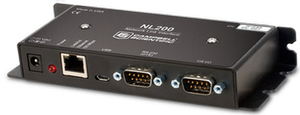
\includegraphics[width=200pt]{images/nl200}
        \caption{Periférico Campbell NL200}
	\label{nl200} 
\end{figure}

Como característica adicional hay que señalar que es un periférico diseñado especialmente para funcionar con el ''datalogger'' antes mencionado y además es un periférico pensado para un consumo de energía muy bajo, lo que lo hace ideal para estar conectado a la batería de la estación. Sus características principales son:

\begin{itemize}
\item Conector de corriente: DC Barrel.
\item Requerimientos de corriente: 7 to 20 Vdc. 
\item Consumo de corriente: 50 mA active @ 13 Vdc.
\item Standby forzado al tener 2 mA de corriente cuando esta conectado al puerto CS I/O en modo Bridge.
\item Rango de temperatura en operación : ${-25}^{\circ}$ to ${+50}^{\circ}C$.
\item Puede ser configurado a través de USB o Ethernet, mediante Telnet.
\item Puerto CS I/O: SDC 7, 8, 10, or 11.
\item Puerto RS-232: DTE.
\item Puerto USB: Micro-B.
\item Puerto Ethernet: IEEE 802.3, Auto-MDIX, IPv4, TCP, DHCP, Ping, Telnet, TLS, PakBus.
\item Dimensiones: 16 x 6.73 x 2.54 cm.
\item Peso: 177 g.
\item Puerto RS-232 DTE: 1200 hasta 115.2k bps.
\item Puerto CS I/O: 9600 hasta 460.8k bps.
\item Ethernet: 10/100 Mbps.
\end{itemize}

\paragraph{MultiModem Multitech modelo MTCBA-G-F4:}
Este periférico construido y distribuido por Multitech\cite{hardware:multitech} es un módem que permite conectarse a una red GSM y/o GPRS, funciona en conjunto con el ''datalogger'' Campbell de la misma forma que lo hace el periférico NL200, salvo que este módulo provee al ''datalogger'' de una conexión a Internet de manera inalámbrica a través de la red de telefonía celular, permitiendo conectar estaciones de monitoreo en lugares remotos (Ver Fig:\ref{modem}).\\

\begin{figure}[h!]
        \centering
        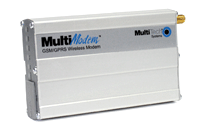
\includegraphics[width=200pt]{images/MultiModemGPRS}
        \caption{MultiModem Multitech MTCBA-G-F4}
	\label{modem} 
\end{figure}

Para poder operar con este módem, es necesario contar con un plan de datos contratado de telefonía móvil con alguna de las compañías que operan en el sector donde se instalan las estaciones de monitoreo. Sus características principales son:\\

\begin{itemize}
\item GPRS Clase 10.
\item Banda cuádruple GSM 850/900/1800/1900 MHz.
\item Corrección de errores MNP 2, Compresión V.42-bis.
\item transmisión de datos hasta 85.6K bps.
\item Pila TCP/IP embedida.
\item Conector de antena SMA.
\end{itemize}

\paragraph{Piranómetro PSP-Eppley:}
El Piranómetro de Precisión Espectral, es un instrumento de medición de clase mundial designado para medir la radiación entregada por el sol y la atmósfera para todo el espectro eléctrico. Se compone de una multi-unión circular de hilo bobinado junto a una termo-pila Eppley que tiene la capacidad de soportar fuertes vibraciones y choques mecánicos (Ver Fig:\ref{piranometro}).

\begin{figure}[h!]
        \centering
        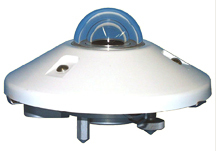
\includegraphics[width=150pt]{images/piranometro}
        \caption{Piranómetro psp-eplay}
	\label{piranometro}
\end{figure}

\paragraph{Sensor de temperatura y humedad HMP60:}
Es una sonda de humedad sencilla, económica y duradera. Es adecuada para aplicaciones de volumen, integración en equipos de otros fabricantes, incubadoras, cajas de manipulación con guantes, invernaderos, cámaras de fermentación y registradoras de datos (Fig:\ref{hr}).

\begin{figure}[h!]
        \centering
        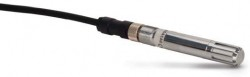
\includegraphics[width=200pt]{images/SensorThmp60}
        \caption{Sensor HMP60}
	\label{hr}
\end{figure}

\paragraph{Batería PS100 Campbell Sci:}
Baterías de plomo-ácido, la fuente de alimentación cuenta con un regulador de carga, puertos libres con salidas DC 12V, además de un conector para el módulo fotovoltaico.

\newpage
\begin{figure}[h!]
        \centering
        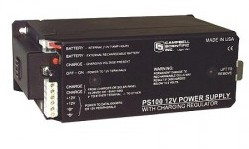
\includegraphics[width=170pt]{images/bateria}
        \caption{Batería PS100} 
\end{figure}

\paragraph{Panel fotovoltaico SX310M:}
Módulo fotovoltaico de alta eficiencia, compuesto por celdas de nitrito de silicio policristalinas.

\begin{figure}[h!]
        \centering
        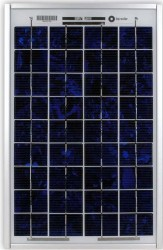
\includegraphics[width=90pt]{images/panelSolar}
        \caption{Panel Solar SX310M} 
\end{figure}

Sus características principales son:
\begin{itemize}
\item Tensión: 12.00 V.
\item Potencia: 10 W.
\item Corriente de salida: 0.59 mA.
\item Largo: 26.9 cm.
\item Alto: 42.1 cm.
\item Grosor: 2.3 cm.
\item Peso: 1.49 Kg.
\end{itemize}

\newpage
\section{Diseño de la solución}
Basándonos en el análisis de la sección \ref{arquitectura} se diseñó una solución de 3 componentes, las cuales podemos apreciar de manera más clara en el Diagrama de Despliegue (Fig:\ref{diagramaDespliegue}). Este diagrama detalla de manera precisa la implementación que tiene cada uno de los componentes.\\

\begin{figure}[h!]
        \centering
        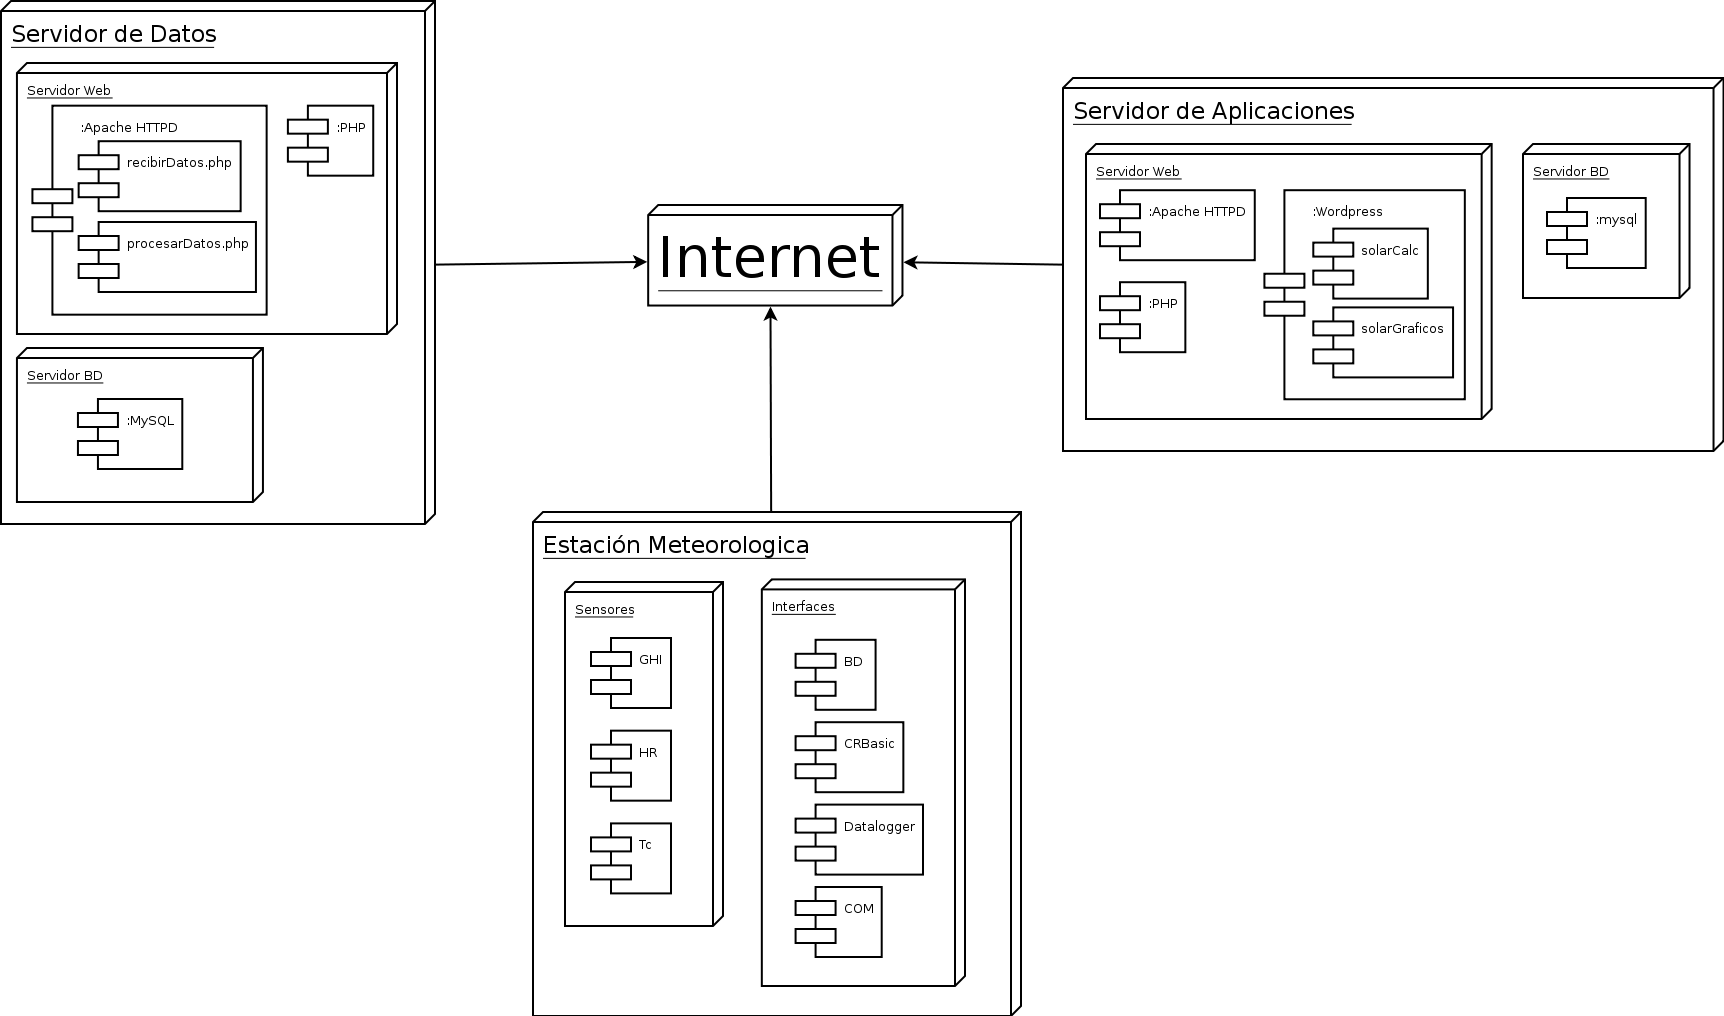
\includegraphics[width=15cm,height=12cm]{images/despliegue}
        \caption{Diagrama de Despliegue.}
	\label{diagramaDespliegue}
\end{figure}

\subsection{Servidor de Aplicaciones}
En el componente de ''Aplicaciones'' se distinguen 3 partes, en primer lugar el ''Sitio Web de la RedSolLAC'', el cual fue desarrollado con anterioridad al inicio de esta memoria, la segunda parte es el módulo ''solarGraficos'' que permite visualizar los datos originados por las estaciones meteorológicas y finalmente el módulo ''solarCalc'', el cual consiste en una calculadora para dimensionar sistemas fotovoltaicos, que junto al módulo de datos y los parámetros ingresados por el usuario entrega un informe de producción energética.

\begin{figure}[h!]
        \centering
        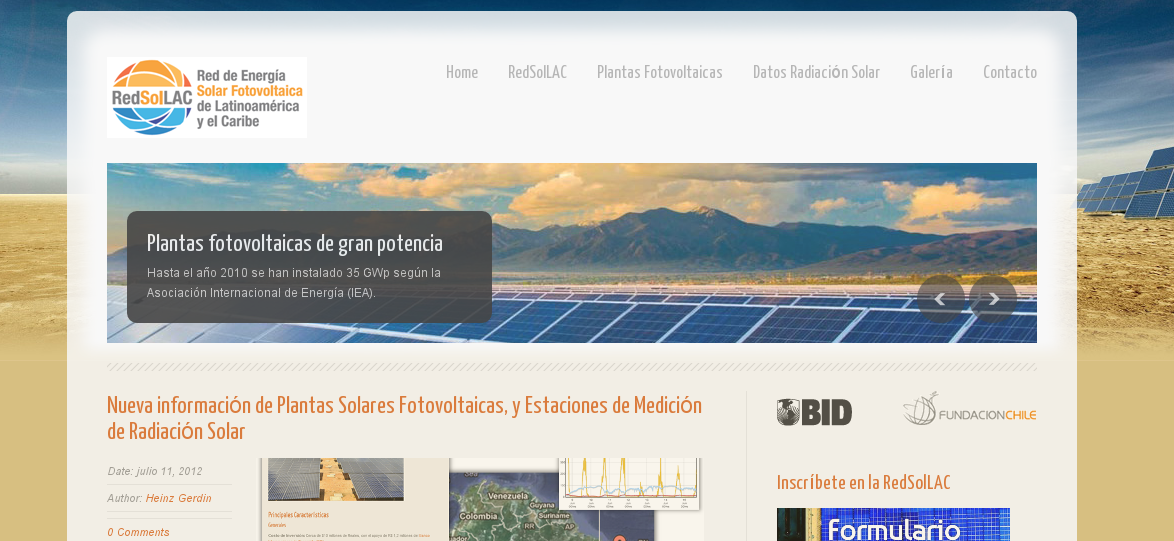
\includegraphics[scale=0.3]{images/webRedSolLAC}
        \caption{Sitio Web RedSolLAC}
        \label{webRed}
\end{figure}

\subsubsection{Sitio web RedSolLAC}
Inicialmente, antes de desarrollar esta Memoria, RedSolLAC desarrolló un sitio web (Ver Fig:\ref{webRed}) el cual le proporcionó una herramienta de difusión. En un principio no requería de un sistema de publicación Web complejo, necesitaba un sistema que le permitiese agregar nuevas noticias e información, así como de administrar la parte visual, estos requerimientos condujeron a la implementación del CMS Wordpress. Posteriormente RedSolLAC se vio en la necesidad de implementar nuevas herramientas innovadoras que pudiesen generar curiosidad en sus usuarios antiguos así como en los futuros usuarios que tendría la Red.\\
Las características del sitio sobre el cual se implementan las mejoras planteadas en esta solución son:
\begin{table}[h!]
\caption{Características sitio Web RedSolLAC}
\resizebox{15cm}{!}{
\begin{tabular}{| c | p{11cm} |}
        \hline
        \textbf{}  &       \textbf{}        \\
        \hline
	Wordpress&Versión 3.4.1\\
	\hline
	Theme(Perfil)&Revelation V1.0\\
	\hline
	Plugins&Contact(v0.7.1), Custom sidebars(v1.1), Google Analytics(v1.0.2), Maintenance Mode(v5.4), WordPress Google Form(v0.3), Wordpress Importer(v0.6)\\
	\hline
	Hosting&Godaddy.com, Deluxe Linux, 150Mb, 500 Email, Ancho de banda ilimitado, 25 BD Mysql, DNS, 50 cuentas FTP\\
	\hline
	Base de datos&versión 5.0\\
	\hline
	PHP&Versión 5.2\\
	\hline
	Dominio&redsollac.org\\
	\hline
\end{tabular}
}
\end{table}

\newpage
\subsubsection{SolarGraficos}
''SolarGraficos'' es el nombre de la primera aplicación desarrollada en esta Memoria y que cumple con los requerimientos de exponer los datos de manera sencilla e intuitiva capturados por las estaciones meteorológicas, en el sitio web de RedSolLAC. Esta aplicación fue desarrollada en PHP 5 y complementada con JavaScript y jQuery, adicionalmente utiliza la biblioteca Flot para crear un gráfico que incluye las mediciones individuales de los siguientes parámetros: radiación global horizontal(GHI), temperatura ambiente(Tc) y humedad relativa del aire(HR).\\

La aplicación fue desarrollada siguiendo la estructura de programación de plugins de Wordpress\cite{aplicacion:wplugins}, usando las funciones de la API que registran y eliminan gatilladores en tiempo de ejecución. El ''plugin'' creado registra una nueva ''pagina de Wordpress'' la cual utilizando una llamada ''Ajax'' solicita la ejecución del fichero ''solarGrafico.php''. Este fichero contiene el código esencial que conforma la aplicación.\\

En primera instancia ''solarGrafico.php'', desde el lado del servidor, crea la estructura estática de la aplicación y escribe el código ''JavaScript'' que permite luego en tiempo de ejecución del lado del cliente hacer las llamadas necesarias que muestran los datos solicitados (Ver Fig:\ref{solarGraficoFoto1}). Una vez creada la estructura de la página se solicita al ''Servidor de Almacenamiento de datos'' mediante una consulta ''Ajax'' sincrónica, los datos del período ''día'', el cual es el período por defecto. Una vez que estos datos están completamente cargados, la aplicación crea un gráfico por defecto que contienen las 3 curvas mencionadas con anterioridad (GHI, HR y Tc) para el periodo del día actual. Luego de crear el gráfico se cargan las barras que muestran la última lectura de cada parámetro y el módulo de descarga de datos. Finalizada esta carga inicial, el sistema ejecuta 3 llamadas ''Ajax'' asincrónicas (Ver Fig:\ref{solarGraficoS}) al ''Servidor de Almacenamiento de Datos'' solicitando datos de los períodos correspondientes (semana, mes y año) tomando como referencia la fecha actual. A medida que los datos se cargan, la opción de visualizar dicho período va apareciendo como disponible en la interfaz de usuario para que éste pueda solicitar sea graficada. Gracias a que las llamadas para cargar los datos de los períodos de tiempo más extensos son llamadas asincrónicas, el navegador no se bloquea y el usuario puede seguir utilizando la aplicación. (Ver Fig:\ref{solarGraficoE}).

\begin{figure}[h!]
        \centering
        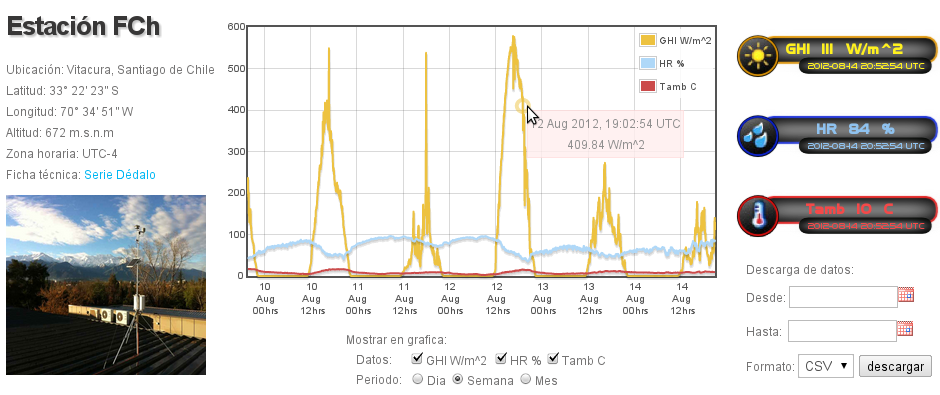
\includegraphics[scale=0.45]{images/solarGrafico}
        \caption{Imagen de la aplicación SolarGraficos}
        \label{solarGraficoFoto1}
\end{figure}

\newpage
\begin{figure}[h!]
        \centering
        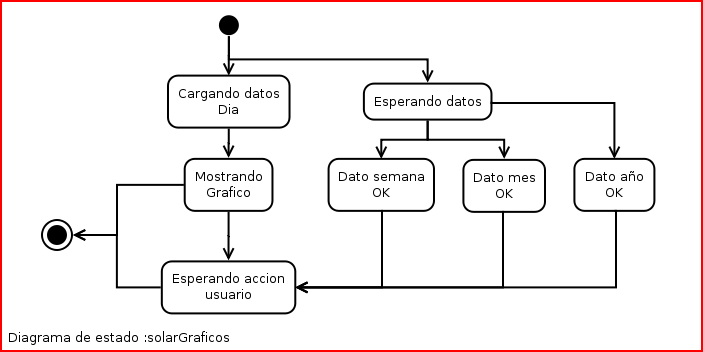
\includegraphics[scale=0.5]{images/graficosEstados}
        \caption{Diagrama de Estados solarGraficos}
        \label{solarGraficoE}
\end{figure}

\begin{figure}[h!]
        \centering
        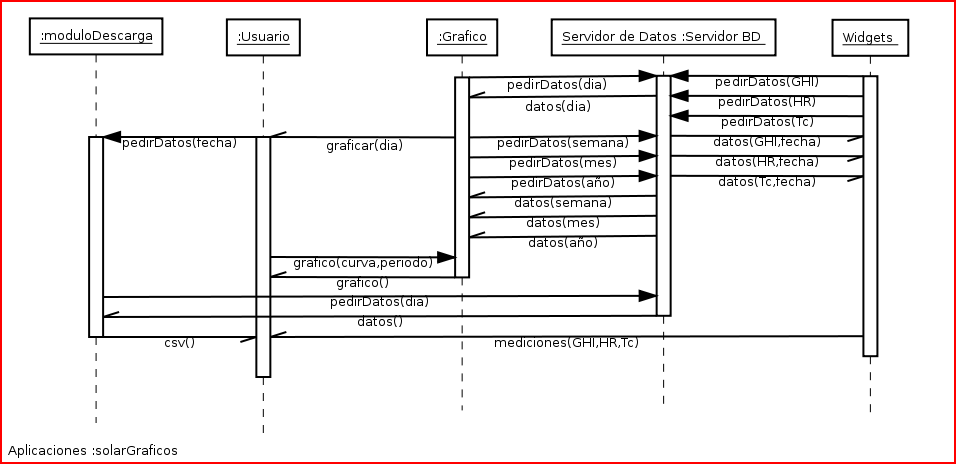
\includegraphics[scale=0.35]{images/graficosSecuencia}
        \caption{Diagrama de Secuencia solarGraficos}
        \label{solarGraficoS}
\end{figure}

\newpage
\subsubsection{SolarCalc}
''solarCalc'' es el nombre que se le ha asignado a la segunda aplicación desarrollada en esta Memoria. Su función, es recopilar información del usuario referente al tipo de planta fotovoltaica que le gustaría instalar y a la ubicación donde se planea construir. Luego, tomando los datos, realiza un proceso de cálculo descrito más adelante, para finalmente entregar un informe de producción energética. Este informe puede ser utilizado posteriormente en la planificación económica de la futura planta solar.\\

Para el proceso de cálculo, fue necesario modelar un sistema basado en mediciones horarias, es decir para calcular la radiación total en un mes dado, se utiliza un conjunto de datos de GHI de media mensual por un periodo de una año, con estos datos se construye una muestra horaria basada en un modelo de distribución estadístico, obteniendo una cantidad de radiación en $W/m^2$ día para cada mes del año. Este modelo permite aplicar una serie de correcciones y mejoras a los modelos típicamente usados, basados en medias mensuales simples, ya que permite aplicar correcciones diarias en cuanto a los modelos de nubosidad, diferentes parámetros climáticos y características de la luminosidad solar. Este modelo también se sustenta en el comportamiento cíclico del movimiento del Sol y la Tierra que originan el día y la noche, además de las estaciones invierno y verano.\\

Por otra parte, este modelo considera una serie de variables ambientales que influyen en el cálculo de la radiación total recibida en la superficie de los paneles solares. Las variables más importantes que influyen en este cálculo son:

\paragraph{Temperatura ambiente:}
Esta variable altera directamente la eficiencia de conversión de los paneles solares(Ver Anexo:\ref{simpvsistmm}), mientras más calientes se encuentren éstos, menor será su rendimiento. La magnitud de la influencia de la temperatura depende de cada fabricante, el cual incluye en las especificaciones ecuaciones para calcular esta perdida.

\paragraph{Velocidad del viento:}
La velocidad del viento, afecta directamente a la temperatura del panel. Todo objeto expuesto al viento esta afecto a una perdida de calor, este fenómeno se conoce en física como convección. 

\paragraph{Época del año:}
La época del año influye en la cantidad de radiación que reciben los paneles durante el día. En verano esta radiación será más alta y en invierno disminuye. Además, se considera el ángulo que forma la posición del sol respecto del sistema fotovoltaico, donde en verano será más elevada y el tiempo de exposición más largo (más horas de luz durante el día), mientras que en invierno el ángulo formado será menor por lo que las horas de luz serán considerablemente inferiores. Existen además ciertas optimizaciones que pueden ser aplicadas al sistema, tales como la modificación del ángulo de inclinación, menor en verano y mayor en invierno.

\paragraph{Ubicación Geográfica:}
La ubicación geográfica del sistema instalado influye de varias maneras. En primer lugar, la orientación de paneles solares que para un óptimo funcionamiento debe estar mirando hacia el sur en el hemisferio norte y mirando al norte en el hemisferio sur. Además es importante considerar si el sistema estará ubicado en una zona costera, la cual influirá directamente en la proporción de radiación directa, difusa y reflejada. Es importante notar que para obtener resultados óptimos, la inclinación de los paneles respecto de la horizontal del piso, por lo general debe ser parecida a la latitud geográfica en valor absoluto, así tendríamos que ubicar los paneles casi en posición horizontal cuando el sistema se ubique cercano a la línea del Ecuador(paralelo 0) y en posición vertical cuando instalemos sistemas cercanos a los polos(paralelo 90).

\paragraph{Nubosidad:}
El índice de nubosidad influye, en el tipo de radiación que reciben los paneles solares, de acuerdo a lo explicado en el capítulo \ref{solar} si la cantidad de nubes es muy alta, la probabilidad de recibir radiación directa es muy baja, mientras que la redición difusa será en proporción más elevada. Además las nubes evitan que la radiación alcance la superficie, por lo que una gran cantidad de ellas no será beneficioso para la producción de energía. Lo más común es que para hacer este cálculo se utilice un modelo proporcional respecto de la cantidad de radiación extraterrestre y la cantidad de radiación recibida en la superficie de la tierra.

\paragraph{Tipo de superficie:}
Otro factor no tan significativo, pero no menos despreciable, será el tipo de terreno donde se encuentre instalado el sistema. Recordemos que de acuerdo a la composición de la radiación global vista en el capítulo \ref{solar}, una de las componente de ésta, corresponde a la cantidad de radiación que refleja el suelo, entonces tenemos que para una superficie negra la absorción será total y no reflejará parte alguna (ej. tierra). Mientras que una superficie blanca, reflejará prácticamente toda la radiación, resultando muy beneficiosa (ej. nieve).\\

Como se mencionó en el párrafo anterior, las variables que afectan la producción de energía solar son muchas y cada una más compleja que la anterior, por lo que la versión de la calculadora que se publica con esta memoria solo incluye algunos de los parámetros más relevantes para este cálculo (época del año, ubicación geográfica, nubosidad, tipo de superficie ), dejando los otros para futuras mejoras (temperatura ambiente).\\

A medida que la RedSolLAC se haga más conocida, tendrá acceso a mayor cantidad de datos empíricos, por lo que el modelo predictivo podrá ir desapareciendo para dar paso a un cálculo basado en datos reales.\\

Los siguientes diagramas, de secuencia (Ver Fig. \ref{solarCalcS}) y estado (Ver Fig. \ref{solarCalcE}), respectivamente exponen el funcionamiento de la calculadora.

En el anexo \ref{phpCalculadora} se puede ver el ''script'' en PHP que realiza los cálculos.\\

\begin{figure}[h!]
        \centering
        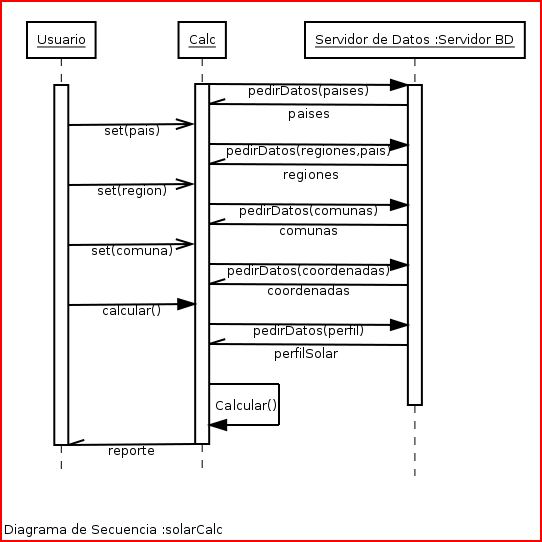
\includegraphics[scale=0.4]{images/calcSecuencia}
        \caption{Diagrama de Estados solarCalc}
        \label{solarCalcS}
\end{figure}
\begin{figure}[h!]
        \centering
        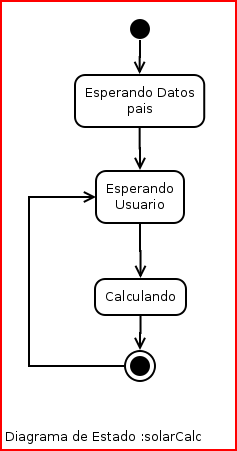
\includegraphics[scale=0.4]{images/calcEstado}
        \caption{Diagrama de Secuencia solarCalc}
        \label{solarCalcE}
\end{figure}

\newpage
\subsection{Estaciones meteorológicas}
La componente ''Estaciones meteorológicas'', abarca todas las estaciones de medición que están adaptadas para registrar datos en el ''Servidor de almacenamiento de datos'', para ello fue necesario acondicionar cada estación, agregándoles un módulo de comunicación, este módulo de comunicación depende del lugar geográfico donde se ubica la estación, ya que esto determinará la tecnología a implementar. Cualquiera sea la tecnología, ésta debe permitir que cada estación se conecte a Internet y a través de esta red pueda, contando con las debidas llaves de autenticación, acceder al ''servidor de almacenamiento de datos''. Adicionalmente y para dar cumplimiento a los requerimientos de seguridad y resguardo de datos, fue necesario programar el módulo para que pudiese almacenar datos de manera local, independiente del estado de la conexión, diseñando un protocolo manual de restauración de datos, previniendo de esta forma, posibles pérdidas de datos.\\

Principalmente, Fundación Chile, ofrece a sus clientes dos tipos de estaciones, serie ''Dédalo'' y serie ''Icaro'', cada una de ellas tienen componentes diferentes y fueron diseñadas para diferentes propósitos, las especificaciones generales de cada una de las series se encuentra en la sección de anexos (Dédalo Ver: \ref{dedalo} e Icaro Ver: \ref{icaro}). Para realizar las pruebas del sistema se utilizó una estación serie Dédalo, que es la estación ubicada en la comuna de Vitacura en las instalaciones de Fundación Chile. Las características específicas de esta estación se presentan en el cuadro siguiente:

\begin{table}[h!]
\label{estacionDedalo}
\caption{Características específicas estación Dédalo Fundación Chile}
\begin{tabular}{| c | p{9cm} |}
        \hline
        \textbf{Componente}  &       \textbf{Detalle}        \\
        \hline
	Datalogger&Campbell Sci. CR1000\\
	\hline
	Piranómetro&Apogee 10.1\\
	\hline
	Sensor de Humedad&HMP60 Vaisala\\
	\hline
	Sensor de Temperatura&HMP60 Vaisala\\
	\hline
	Interfaz de Comunicación&Campbell Sci NL200\\
	\hline
\end{tabular}
\end{table}

Para que dicha estación opere de manera correcta es necesario programar su ''datalogger'' con un ''script'' escrito en CRBasic. Este script se encuentra en la sección de anexos (Ver: anexo \ref{getData}).\\

Inicialmente el ''script'' contiene la definición de variables que utilizará durante la ejecución, son tanto las variables de ejecución como las que serán posteriormente referenciadas a los diferentes ''inputs'' de cada sensor.\\
Luego sigue la definición de unidades. Cada instrumento mide parámetros en magnitudes físicas diferentes y el lenguaje permite declarar estas unidades.\\
En tercer lugar se declara la definición de tablas de datos que almacenan los datos capturados por los instrumentos conectados. Pueden ser declaradas tantas tablas como sea necesario, sin embargo, a cada una se le debe asignar la cantidad de registros máxima que puede almacenar. En el eventual caso en que sea necesario más de una tabla, se debe planificar bien el uso de la memoria, ya que es un recurso limitado en el ''datalogger''.\\
Como cuarto elemento, se da inicio a la ejecución del ''script'' con la declaración ''BeginProg'' y ''Scan''. Esta última declaración será una rutina de ejecución iterativa en el tiempo, parámetro que debe ser declarado en la misma instrucción.\\
Dentro de la declaración ''Scan'', se establece una nueva conexión TCP/IP mediante la apertura de un ''socket'', si la conexión es exitosa, se envían los datos mediante la instrucción ''GET'', si no, saltamos dicho paso. Finalmente se almacenan los datos medidos en la tabla de memoria interna.\\

Para graficar de mejor manera cuál es el comportamiento de la estación se presenta un diagrama de estados y un diagrama de secuencia (Ver Fig: \ref{estacionEstados} y \ref{despliegue}).

\begin{figure}[h!]
        \centering
        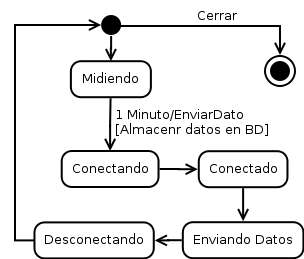
\includegraphics[scale=0.6]{images/estacionEstados}
        \caption{Diagrama de Estado estación meteorológica}
        \label{estacionEstados}
\end{figure}

\begin{figure}[h!]
        \centering
        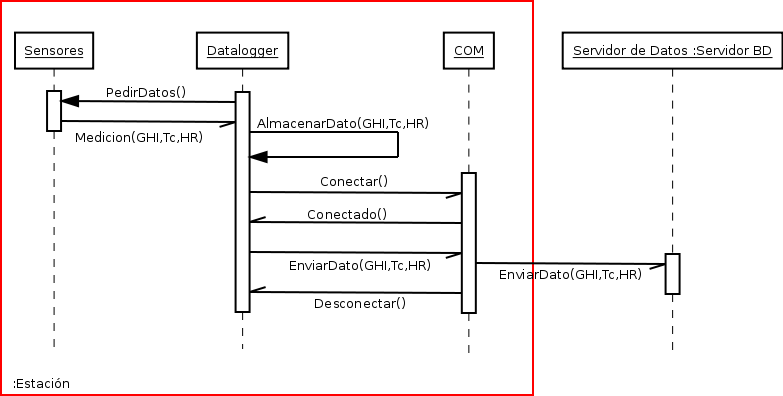
\includegraphics[scale=0.5]{images/estacionSecuencia}
        \caption{Diagrama de Secuencia estación meteorológica}
        \label{despliegue}
\end{figure}

\subsection{Servidor de almacenamiento de datos}
Anterior al desarrollo de este sistema, cada estación almacenaba datos en su memoria interna y era necesario que una persona accediese físicamente a cada estación con un PC portátil a descargar los datos. Este proceso resultaba bastante complejo y en varias ocasiones se perdían datos.\\
Esta nueva componente cuenta con un servidor de bases de datos y un servidor Web, el cual es utilizado para el manejo y mantención de la base de datos y el control de acceso.\\

El sistema de ''Almacenamiento de Datos'' está compuesto por un solo servidor físico, el cual implementa el servidor Web Apache HTTPD y el servidor de bases de datos MySQL. El servicio MySQL se encarga directamente de almacenar los datos que llegan desde las estaciones y atender las solicitudes de datos del ''servidor de aplicaciones'', mientras que el servicio Web implementa ciertas rutinas escritas en PHP que componen el sistema de seguridad e integridad de los datos. Adicionalmente implementa rutinas que forman parte del sistema de respaldo manual para casos de falla del sistema.\\

Uno de los requerimientos claves de este sistema es la robustez e integridad de los datos, así como la confiabilidad de ellos. Este sistema tiene restringido el ingreso de datos solo al módulo de estaciones y en ocasiones especiales al sistema de mantenimiento manual, por lo que implementa rutinas en PHP, a través del servidor Web que impiden que cualquier actor diferente de una estación pueda registrar datos nuevos. Estas rutinas son ejecutadas directamente por las estaciones a través del ''datalogger'' haciendo llamadas GET con las llaves de seguridad adecuadas.\\

El sistema implementa una salida de datos libre, esto quiere decir que cualquiera que posea acceso a la base de datos puede solicitar el envío de éstos a sus aplicaciones sin la necesidad de llaves extras de seguridad. Este acceso está pensado para que los datos sean publicados a través de las aplicaciones desarrolladas en cualquier sitio, incluido el sitio de la RedSolLAC.\\

Cuando una estación hace una llamada GET, el servidor Web mediante una rutina en PHP verifica las llaves de seguridad e integridad de los datos que le son enviados de la estación para luego enviarlos a la base de datos. Una vez que la petición GET es recibida, ésta devuelve a la estación un mensaje ''200'' si la llamada fue recibida o un mensaje ''404'' si se produjo un error. En cualquier caso para el ''datalogger'' es indiferente si la petición fue aceptada y el sistema no fue diseñado para realizar esta verificación.\\ En una futura implementación, queda planteada la posibilidad de diseñar un protocolo de comunicación que permita la verificación de datos como una forma de mejorar la robustez del sistema.\\

El siguiente diagrama de estados detalla de forma técnica el comportamiento de esta componente:
\begin{figure}[h!]
        \centering
        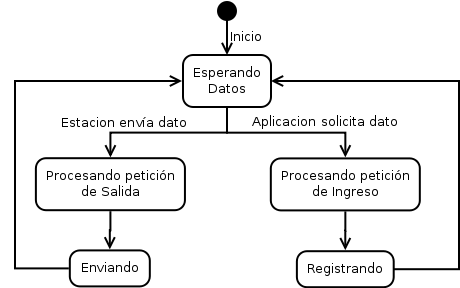
\includegraphics[scale=0.6]{images/datosEstados}
        \caption{Diagrama de Estados Sistema de Almacenamiento}
        \label{almacenamientoSecuencia}
\end{figure}

\subsection{Modelo de datos}
El modelo de datos desarrollado (Ver Fig. \ref{modeloDatos}) cuenta con dos bases de datos, la primera de ellas contiene las tablas de uso general del sistema con información respecto de la radiación solar, datos meteorológicos, información geográfica para las diferentes comunas, información respecto de las estaciones meteorológicas registradas e información de utilidad para la parte gráfica propia del sitio.\\ La segunda base de datos está orientada solo a la recopilación de datos de las diferentes estaciones.\\ Esta decisión, de separar las bases de datos, fue una decisión de diseño del sistema ya que según los requerimientos, cada estación registra parámetros distintos dependiendo de los sensores, si bien hubiese sido posible estandarizar una tabla con la mayoría de los instrumentos, hubiese tenido un tamaño, desde el punto de vista del DBA, inmanejable. Por otro lado, la mayoría de las estaciones registran datos cada un minuto, esto desemboca en un crecimiento muy rápido en la cantidad de registros de las tablas, si bien el crecimiento es lineal en el tiempo, la combinación de registros con todos los sensores posibles, más todas las estaciones juntas en una sola tabla, podrían provocar eventualmente un colapso y grandes dificultades de administración y mantención.\\

Para tener una idea aproximada del crecimiento de las tablas de datos, se plantea el siguiente ejercicio: Solo la estación ''Fundación Chile Vitacura'' almacena en su tabla de datos 3 mediciones (rad\_w, rh, Temp\_tc) más 3 columnas extras para todo registro (id, timestmp, Battv). Además registra datos con intervalos de un minuto, solo esta estación crece 34 MB al año y 525.000 registros al año.

\begin{table}[h!]
\caption{Crecimiento anual de la base de datos}
\begin{tabular}{| c | p{11cm} |}
        \hline
        Numero de columnas & 6\\
        \hline
	Tamaño de la fila & 66 Bytes\\
	\hline
	Cantidad de registros & 525.600 registros\\
	\hline
	Tamaño BD & 33.877 KBytes\\
	\hline
\end{tabular}
\end{table}

A primera vista el tamaño de crecimiento en Bytes no es significativo, considerando la capacidad que manejan los servidores de datos en la actualidad, sin embargo la cantidad de registro ingresados día a día a la base de datos, bajo el supuesto de que existirán un número considerable de estaciones, hace que una sola tabla sea poco manejable ante eventuales o emergencias, tales como fallas del servidor, cortes de electricidad, fallas de discos, etc.

\begin{figure}[h!]
        \centering
        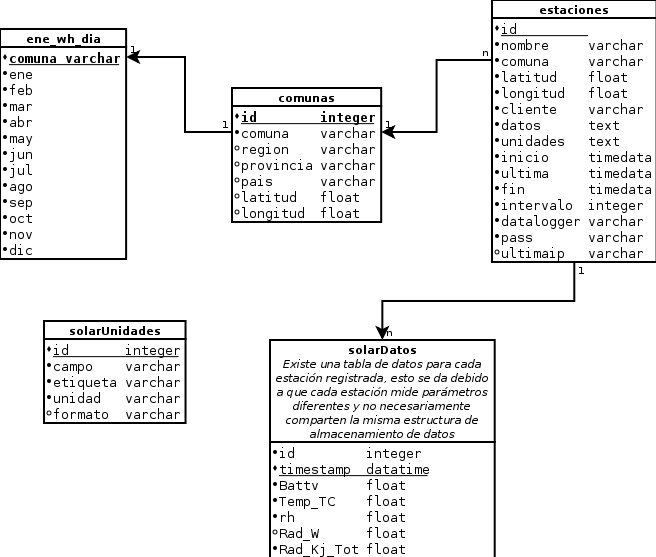
\includegraphics[scale=0.6]{images/modeloDatos}
        \caption{Diagrama del modelo de datos}
        \label{modeloDatos}
\end{figure}


